\documentclass[tikz,border=6pt]{standalone}
\usepackage[T1]{fontenc}
\usepackage[utf8]{inputenc}
\usepackage{amsmath,amssymb}
\usepackage{tikz}
\usetikzlibrary{automata,positioning,arrows.meta,shapes.geometric,calc,fit}
\tikzset{
    >=Stealth,
    every state/.style={minimum size=8mm, inner sep=1pt, font=\small},
    flow/.style={rectangle, rounded corners, draw, align=center, minimum width=3.1cm, minimum height=0.9cm},
    decision/.style={diamond, draw, aspect=2.0, align=center, inner sep=1.5pt},
    terminal/.style={ellipse, draw, align=center, minimum width=2.4cm, minimum height=0.85cm},
    module/.style={rectangle, draw, rounded corners, align=center, minimum width=3.4cm, minimum height=1.0cm},
    data/.style={rectangle, draw, align=center, minimum width=3.2cm, minimum height=0.9cm}
}
\begin{document}
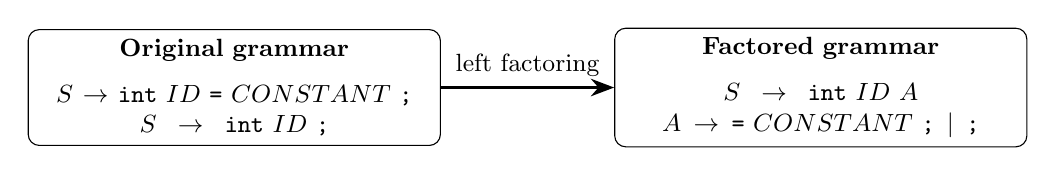
\begin{tikzpicture}[node distance=22mm, font=\small]
    \node[flow, text width=5.0cm] (original) {
        \textbf{Original grammar}\\[2mm]
        $S \rightarrow \texttt{int}\ ID\ \texttt{=}\ CONSTANT\ \texttt{;}$\\
        $S \rightarrow \texttt{int}\ ID\ \texttt{;}$
    };
    \node[flow, text width=5.0cm, right=of original] (factored) {
        \textbf{Factored grammar}\\[2mm]
        $S \rightarrow \texttt{int}\ ID\ A$\\
        $A \rightarrow \texttt{=}\ CONSTANT\ \texttt{;} \mid \texttt{;}$
    };
    \draw[->, very thick] (original) -- node[above] {left factoring} (factored);
\end{tikzpicture}
\end{document}
